\documentclass[a4paper, 11pt]{article}
\usepackage[english]{babel}

\usepackage[top=2.5cm,bottom=2.5cm,left=2cm,right=2cm,marginparwidth=1.75cm]{geometry}



\usepackage{graphicx}
\usepackage{amsmath}
\usepackage{xcolor}
\definecolor{custom-blue}{RGB}{0,99,166} 
\usepackage{hyperref}
\hypersetup{colorlinks=true, allcolors=custom-blue}
\usepackage[default]{sourcesanspro}
\usepackage[T1]{fontenc}
\usepackage{fancyhdr}
\usepackage{titlesec}
\usepackage{makecell}
\usepackage{float}

\usepackage{lastpage}

\usepackage[table,xcdraw]{xcolor}

\usepackage{graphicx}
\usepackage{amsmath}
\usepackage{xcolor} % Standard xcolor
\usepackage{listings} % ADD THIS HERE

% --- Define colors for SQL highlighting ---
\definecolor{codegreen}{rgb}{0,0.6,0}
\definecolor{codegray}{rgb}{0.5,0.5,0.5}
\definecolor{codepurple}{rgb}{0.58,0,0.82}
\definecolor{backcolour}{rgb}{0.95,0.95,0.92}

% --- Configure the listings style ---
\lstset{
    language=SQL,
    backgroundcolor=\color{backcolour},   
    commentstyle=\color{codegreen},
    keywordstyle=\color{custom-blue}, % Use your defined blue
    numberstyle=\tiny\color{codegray},
    stringstyle=\color{codepurple},
    basicstyle=\ttfamily\small,
    breaklines=true,                 
    captionpos=b,                    
    keepspaces=true,                 
    showspaces=false,                
    showstringspaces=false,
    showtabs=false,                  
    tabsize=2,
    frame=single % Adds a nice border around your code
}

\definecolor{custom-blue}{RGB}{0,99,166} 
% ... (rest of your titlesec and fancyhdr setup)




\definecolor{darkblue}{HTML}{365F91}
\definecolor{blue}{HTML}{4F81BD}
\definecolor{darkdarkblue}{HTML}{243F60}

\titleformat{\section}
  {\normalfont\LARGE\upshape\color{darkblue}}{\thesection.}{1em}{}

\titleformat{\subsection}
  {\normalfont\Large\upshape\color{blue}}{\thesubsection.}{1em}{}[{\color{black}\titlerule[0.2pt]}]

\titleformat{\subsubsection}
  {\normalfont\large\upshape\color{blue}}{\thesubsubsection.}{1em}{}[{\color{black}\titlerule[0.2pt]}]

\pagestyle{fancy}
\fancyhf{}
\setlength{\headheight}{30pt}
\renewcommand{\headrulewidth}{0.5pt}
\renewcommand{\footrulewidth}{0.5pt}

\fancyhead[L]{
\includegraphics[width=3cm]{univienna-logo.eps}}
\fancyhead[R]{University of Vienna}
\fancyfoot[R]{\thepage/\pageref{LastPage}}

\newcommand{\studentone}{Student 1:
Trumshi, Ines, 12220438}
\newcommand{\studenttwo}{Student 2: Korobeinikova, Anastasiia, 12248216}
\newcommand{\studentthree}{Student 3: Brayko, Anna, 12343205}

\begin{document}

\begin{figure}
\flushleft

\includegraphics[width=0.4\textwidth]{univienna-logo.eps}
\end{figure}

\title{052400-1 VU Information Management and Systems Engineering (2026S)\\[1em] Milestone 1}
\author{
Group 24\\[1em]
\studentone\\[1em]
\studenttwo\\[1em]
\studentthree
}
\date{April 2026, Vienna}

\maketitle
\newpage
\tableofcontents
\newpage

%%%%%%%%%%%%%%%%%%%%%%%%%%%%%%%%%%%%%%%%%
\section{Milestone 1}

%%%%%%%%%%%%%%%%%%%%%%%%%%%%%%%%%%%%%%%%%
\subsection{Team - Conceptual Modeling}

\subsubsection{Describe the Application Domain}

The application domain is a web-based language learning system focused on learning Norwegian vocabulary. Users are assigned wordlists and individual words, and they interact with the system through learning and reviewing sessions.

The system tracks user progress by storing correct answers, mistakes, and review intervals. Words are grouped into wordlists, and wordlists can be categorized into topics such as food, travel, or daily activities.

The system enables personalized learning by allowing users to filter wordlists by topic and adapting review frequency based on user performance.

\subsubsection{Entities and Relationships}
\begin{table}[H]
\begin{tabular}{|l|l|}
\hline
\rowcolor[HTML]{93C47D}  
\textbf{Requirements} & \textbf{Realization} \\ \hline

\rowcolor[HTML]{D9D9D9}
\textbf{Entities} & \\ \hline

\cellcolor[HTML]{D9D9D9} Users & (user\_id, username, language, preferred\_topic\_id) \\ \hline
\cellcolor[HTML]{D9D9D9} Words & (word\_id, word, translation, difficulty, base\_word\_id) \\ \hline
\cellcolor[HTML]{D9D9D9} Wordlists & (wordlist\_id, name) \\ \hline
\cellcolor[HTML]{D9D9D9} Topics & (topic\_id, name, description) \\ \hline
\cellcolor[HTML]{D9D9D9} User\_Word & (user\_id, word\_id, is\_new, correct\_count, mistakes\_count, next\_review, last\_reviewed, interval) \\ \hline
\cellcolor[HTML]{D9D9D9} Wordlist\_Word & (wordlist\_id, word\_id) \\ \hline
\cellcolor[HTML]{D9D9D9} User\_Wordlist & (user\_id, wordlist\_id, enrolled\_at) \\ \hline
\cellcolor[HTML]{D9D9D9} Weak Entity & User\_Word \\ \hline

\rowcolor[HTML]{D9D9D9}
\textbf{Relationships} & \\ \hline

\cellcolor[HTML]{D9D9D9} Unary & Word -- Word (base\_word\_id for variations) \\ \hline
\cellcolor[HTML]{D9D9D9} 1:n & User -- User\_Word \\ \hline
\cellcolor[HTML]{D9D9D9} m:n & Wordlist -- Word (via Wordlist\_Word) \\ \hline
\cellcolor[HTML]{D9D9D9} m:n & Wordlist -- Topic \\ \hline
\cellcolor[HTML]{D9D9D9} m:n & User -- Wordlist \\ \hline

\end{tabular}
\end{table}

\clearpage

\subsubsection{Logical Design -- ER Diagram in Chen Notation}

\begin{center}

\begin{figure}[h!]
    \centering
    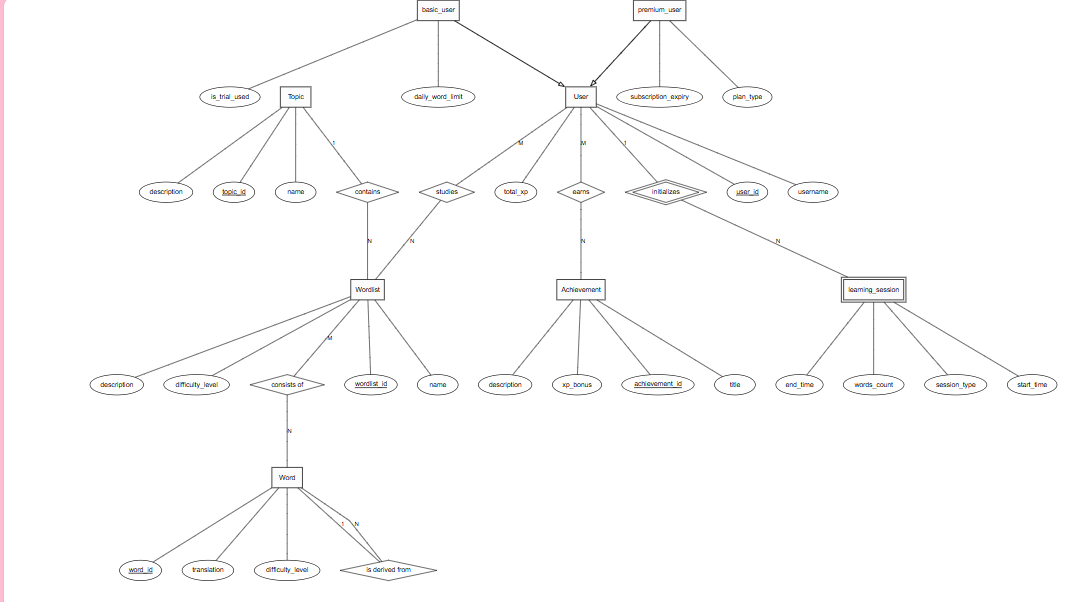
\includegraphics[width=1.1\textwidth]{ER_FINAL.png}
    \caption{ER diagram}
    \label{fig:ecommerce-process}
\end{figure}
\end{center}

\subsubsection{Relational Modeling -- SQL Tables}
\begin{itemize}
  \item \textbf{Users}(user\_id PK, username, language, preferred\_topic\_id FK)
  \item \textbf{Words}(word\_id PK, word, translation, difficulty, base\_word\_id FK)
  \item \textbf{Topics}(topic\_id PK, name, description)
  \item \textbf{Wordlists}(wordlist\_id PK, name, topic\_id FK)
  \item \textbf{Wordlist\_Word}(wordlist\_id PK, word\_id PK)
  \item \textbf{User\_Wordlist}(user\_id PK, wordlist\_id PK, enrolled\_at)
  \item \textbf{User\_Word}(user\_id PK, word\_id PK, is\_new, correct\_count, mistakes\_count, next\_review, last\_reviewed, interval)
\end{itemize}


%%%%%%%%%%%%%%%%%%%%%%%%%%%%%%%%%%%%%%%%%
\newpage
\subsection{Individual - Student 1}
\studentone
\subsubsection{Use Case Definition and Design}
\begin{tabular}{@{}lp{10cm}@{}}
\toprule
\textbf{Use Case Name} & Assign Word to Wordlist (many-to-many) \\
\midrule
\textbf{Trigger} & An user selects one word and adds it
                   to an existing wordlist via the user interface to review it again. \\[4pt]
\textbf{Preconditions} &
  \begin{minipage}[t]{10cm}
    \begin{itemize}
      \item The user is logged in.
      \item At least one \textbf{Wordlist} and at least one \textbf{Topic} exist in
            the system.
      \item The selected word was already viewed at least once by the user.
    \end{itemize}
  \end{minipage} \\[4pt]
\textbf{Main Flow} &
\begin{minipage}[t]{10cm}
\begin{enumerate}
  \item The user starts a review session and reviews a word.
  \item The user identifies the word as difficult.
  \item The user clicks on "Add again to Wordlists".
  \item The frontend sends an API POST request to the backend.
  \item The backend processes the request and updates the database:
  \begin{itemize}
      \item The \texttt{User\_Words} table is updated.
      \item A new entry is inserted into the \texttt{Wordlist\_Words} table to reassign the word to the wordlist.
  \end{itemize}
  \item The backend returns a success confirmation to the frontend.
  \item The system displays a message: “Word added to review again”.
  \item The system asks the user if they want to continue reviewing.
  \item If yes, the next word is displayed and the process repeats.
  \item If no, the review session ends.
\end{enumerate}
\end{minipage} \\[4pt]
\textbf{Postconditions} &
  \begin{minipage}[t]{10cm}
    \begin{itemize}
      \item One or more new rows exist in \texttt{user\_wordlist}.
      \item Users whose word was now again added to the wordlist can know review it again.
    \end{itemize}
  \end{minipage} \\[4pt]
\textbf{Entities} & \textbf{User}, \textbf{Word} , \textbf{Wordlist} 
\bottomrule
\end{tabular}
\clearpage
\paragraph*{Graphical Representation}

\begin{center}
\begin{figure}[H]
    \centering
    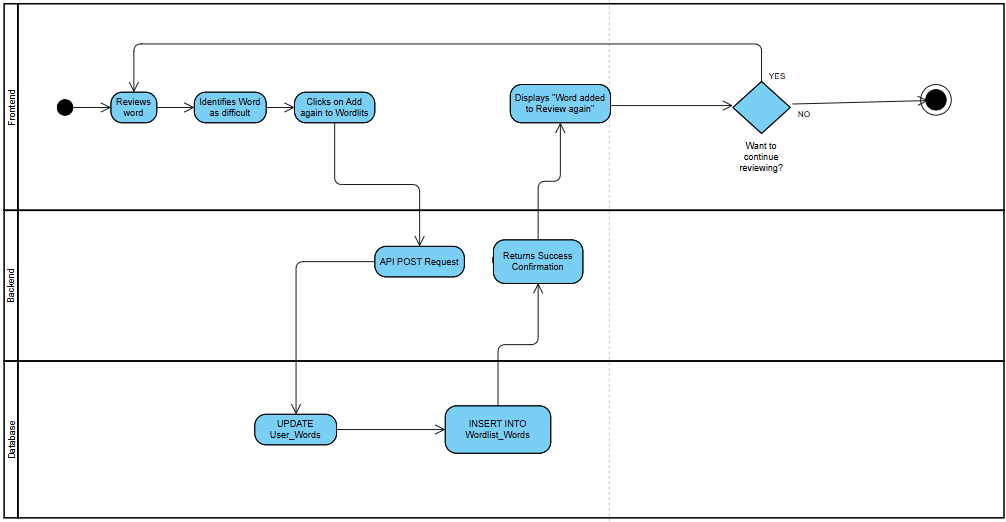
\includegraphics[width=0.8\textwidth]{new_activitydiag_ines.png}
    \caption{Activity Diagram for Use Case 1}
    \label{fig:activity-diagram}
\end{figure}
\end{center}

\subsubsection{Analytics Report}



\subsubsection*{Concept}
 
\noindent\textbf{Report description:}\\
This report identifies which words a specific user has manually flagged for extra practice by adding them to their active wordlists. It allows the system (or the user) to see the most difficult words that have constantly been added and identifying which lists are growing because the user feels they haven't mastered those specific words yet.
 
\medskip
\noindent\textbf{Filter field:} \texttt{username} (e.g.\ \texttt{'MaxMustermann'})
 
\medskip
\noindent\textbf{Entities involved:} \textbf{User}, \textbf{Wordlist}, \textbf{Word}

 
\noindent\textbf{Why results change after the use case executes:}\\
Before execution, the target wordlist is not linked to the users wordlist, because it was already "reviewed", so it does not
appear in the query result. After the use case inserts the row into
\texttt{wordlist}, the word  appears in the
result set for the filtered user.
 
% ---------- Proof of Concept ----------------------------------------
\subsubsection*{Proof of Concept}

As the POC on the use case, we are going to perform different SQL statements and queries on the difficult norwegian word "Melk" (Milk). 
The user has words added to the wordlist for him/her to study.
 
\noindent\textit{Initial Query result}

\begin{center}
\begin{figure}[H]
    \centering
    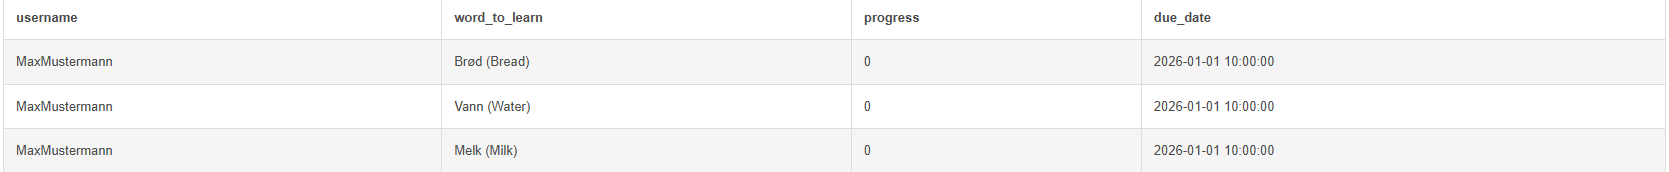
\includegraphics[width=1.0\textwidth]{INSERT_dummy_data_ines.png}
    \label{fig:activity-diagram}
\end{figure}
\end{center}
\\

After the user studied the words we see an empty table when looking for the difficult word "Milk" for the user to review for additional preparation.
\begin{center}
\begin{figure}[H]
    \centering
    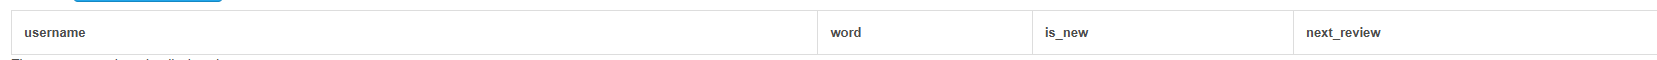
\includegraphics[width=1.0\textwidth]{1_imse.png}
    \caption{Initial state}
    \label{fig:activity-diagram}
\end{figure}
\end{center}

 
\medskip

\medskip
\noindent\textbf{SQL INSERT Statement}
\\
We want with the code above to add for the user with user\_id = 1 the difficult norwegian word with id = 1.

\begin{lstlisting}[caption={SQL INSERT statement}]
UPDATE User_Words 
SET is_new = TRUE, 
    correct_count = 0, 
    `interval` = 0
-- The word with ID = 1 is "Milk"
WHERE user_id = 1 AND word_id = 1;

-- Link the difficult word to the wordlist to review again
INSERT INTO Wordlist_Words (wordlist_id, word_id) 
VALUES (1, 1);
\end{lstlisting}


 
\medskip
\noindent\textit{Query result AFTER execution of the use case: }
The word becomes a "new" one again, being displayed on the wordlist of the user, ready to get reviewed again.



\begin{center}
\begin{figure}[H]
    \centering
    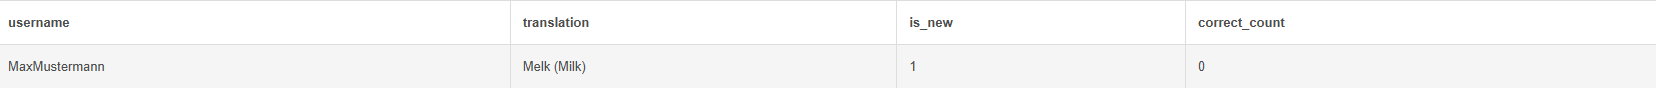
\includegraphics[width=1.0\textwidth]{AFTER_USECASE_ines.png}
    \caption{USE CASE Prove}
    \label{fig:activity-diagram}
\end{figure}
\end{center}

\newpage

\subsection{Individual - Student 2}
\studenttwo
%%%%%%%%%%%%%%%%%%%%%%%%%%%%%%%%%%%%%%%%%
\subsubsection{Use Case Definition and Design}

The use case is assigning new wordlists to the user. Version 3 (many-to-many) is used (user can have many words assigned, and a word can be assigned to many users).

\paragraph*{Textual Description}
\textbf{Use Case Name (weak entity/IS-A relationship/many-to-many):} 
Assigning a wordlist to a user
\\
\textbf{Trigger:} 
 The administrator needs to assign a wordlist to a user, making it available for them in the app
\\
\textbf{Preconditions:}
\begin{itemize}
    \item The user exists in the database
\item The wordlist exists in the database
\item At least one word is associated with the wordlist

\end{itemize}

\\
\textbf{Main Flow:}
\begin{enumerate}
    \item The administrator selects the user and the wordlist
\item An SQL query is run to associate the wordlist with the user
\item A new record is created in the user\_wordlist table (containing the user\_id and wordlist\_id)
\item An SQL query is run to associate words in the wordlist with the user
\item A new record is created in the user\_word table (containing the user\_id and word\_id) for each word in the wordlist
\end{enumerate}

                 
\\
\textbf{Postconditions:}
\begin{enumerate}
    \item New records are created in the user\_wordlist and user\_word table

\item The user can now retrieve the new wordlist and the words it contains

\end{enumerate}


\textbf{Entities:}

user, wordlist, word (+ bridging tables user\_wordlist, user\_word)


\clearpage

\paragraph*{Graphical Representation}

\begin{figure}[H]
    \centering
    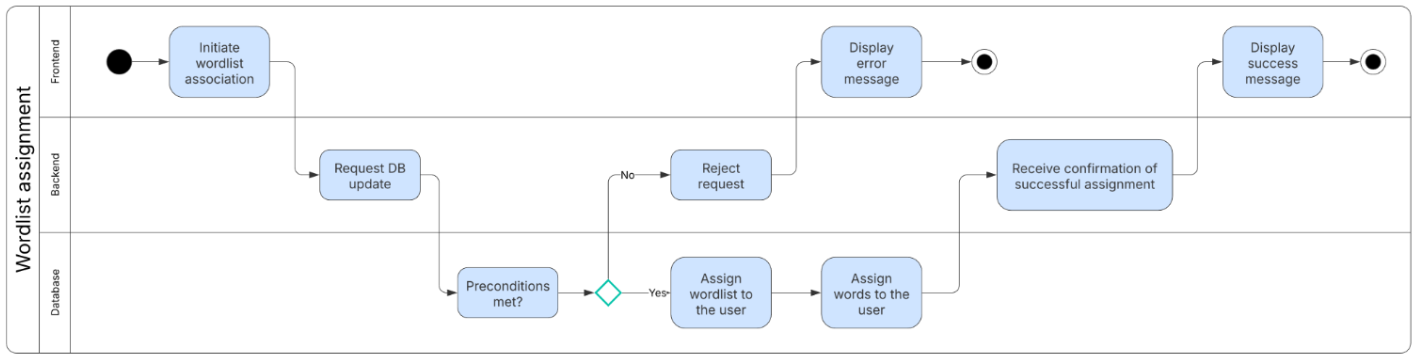
\includegraphics[width=0.8\linewidth]{ans1.png}
    \caption{Activity Diagram Use Case 2}
    \label{fig:placeholder}
\end{figure}


%%%%%%%%%%%%%%%%%%%%%%%%%%%%%%%%%%%%%%%%%
%%%%%%%%%%%%%%%%%%%%%%%%%%%%%%%%%%%%%%%%%
\subsubsection{Analytics Report}
\paragraph*{Concept}
The report lists wordlists and words that have been assigned to the user. This data can be used by the administrator to see what items are available for the user and track learning statistics: when each word was last reviewed and how problematic it is for the user (mistakes and correct answers count).
Filter field: user\_id.
Entities involved: users, words, wordlists + bridging tables user\_words, user\_wordlists, wordlist\_words.
SQL Query:
\begin{verbatim}
    SELECT * FROM user_wordlists WHERE user_id = 1;
    SELECT * FROM user_words WHERE user_id = 1; 
\end{verbatim}

Before execution, the target wordlist and words that it contains are not linked to the target user. After execution, new entries are created in the user\_wordlists and user\_words bridging tables.

Statitics:
\begin{itemize}
    \item 1 new entry in user\_wordlists table
    \item 6 new entries in user\_words table

\end{itemize}

\clearpage


\paragraph*{Proof of Concept }


\paragraph{SQL CREATE statements for tables}
\begin{verbatim}
    MariaDB [LANGUAGE_APP]> CREATE TABLE IF NOT EXISTS Users (
    -> user_id INT UNSIGNED NOT NULL AUTO_INCREMENT PRIMARY KEY,
    -> username VARCHAR(50) NOT NULL,
    -> total_xp INT UNSIGNED DEFAULT 0
    -> );

MariaDB [LANGUAGE_APP]> CREATE TABLE IF NOT EXISTS Topics (
    -> topic_id INT UNSIGNED NOT NULL AUTO_INCREMENT PRIMARY KEY,
    -> name VARCHAR(100) NOT NULL,
    -> description VARCHAR(500)
    -> );

MariaDB [LANGUAGE_APP]> CREATE TABLE IF NOT EXISTS Words (
    -> word_id INT UNSIGNED NOT NULL AUTO_INCREMENT PRIMARY KEY,
    -> word VARCHAR(255) NOT NULL,
    -> translation VARCHAR(255) NOT NULL,
    -> difficulty_level TINYINT UNSIGNED,
    -> base_word_id INT UNSIGNED DEFAULT NULL,
    -> CONSTRAINT fk_word_base FOREIGN KEY (base_word_id)
    -> REFERENCES Words(word_id) ON DELETE SET NULL
    -> );

MariaDB [LANGUAGE_APP]> CREATE TABLE IF NOT EXISTS Wordlists (
    -> wordlist_id INT UNSIGNED NOT NULL AUTO_INCREMENT PRIMARY KEY,
    -> name VARCHAR(100) NOT NULL,
    -> description TEXT,
    -> difficulty_level TINYINT UNSIGNED,
    -> topic_id INT UNSIGNED NOT NULL,
    -> CONSTRAINT fk_wordlist_topic FOREIGN KEY (topic_id)
    -> REFERENCES Topics(topic_id) ON DELETE CASCADE
    -> );

MariaDB [LANGUAGE_APP]> CREATE TABLE IF NOT EXISTS Wordlist_Words (
    -> wordlist_id INT UNSIGNED NOT NULL,
    -> word_id INT UNSIGNED NOT NULL,
    -> PRIMARY KEY (wordlist_id, word_id),
    -> FOREIGN KEY (wordlist_id) REFERENCES Wordlists(wordlist_id) ON DELETE CASCADE,
    -> FOREIGN KEY (word_id) REFERENCES Words(word_id) ON DELETE CASCADE
    -> );

MariaDB [LANGUAGE_APP]> CREATE TABLE IF NOT EXISTS User_Wordlists (
    -> user_id INT UNSIGNED NOT NULL,
    -> wordlist_id INT UNSIGNED NOT NULL,
    -> enrolled_at TIMESTAMP DEFAULT NOW(),
    -> PRIMARY KEY (user_id, wordlist_id),
    -> FOREIGN KEY (user_id) REFERENCES Users(user_id) ON DELETE CASCADE,
    -> FOREIGN KEY (wordlist_id) REFERENCES Wordlists(wordlist_id) ON DELETE CASCADE
    -> );

MariaDB [LANGUAGE_APP]> CREATE TABLE IF NOT EXISTS User_Words (
    -> user_id INT UNSIGNED NOT NULL,
    -> word_id INT UNSIGNED NOT NULL,
    -> is_new BOOLEAN DEFAULT TRUE,
    -> problematic BOOLEAN DEFAULT FALSE,
    -> next_review TIMESTAMP NULL DEFAULT NULL,
    -> last_reviewed TIMESTAMP NULL DEFAULT NULL,
    -> `interval` INT UNSIGNED DEFAULT 0,
    -> correct_count INT UNSIGNED DEFAULT 0,
    -> mistakes_count INT UNSIGNED DEFAULT 0,
    -> last_mistake TIMESTAMP NULL DEFAULT NULL,
    -> PRIMARY KEY (user_id, word_id),
    -> CONSTRAINT fk_uw_user_id FOREIGN KEY (user_id) REFERENCES Users(user_id) ON DELETE CASCADE,
    -> CONSTRAINT fk_uw_word_id FOREIGN KEY (word_id) REFERENCES Words(word_id) ON DELETE CASCADE
    -> );
\end{verbatim}

\paragraph*{SQL INSERT for example data}
\noindent
\begin{figure}[H]
    \centering
    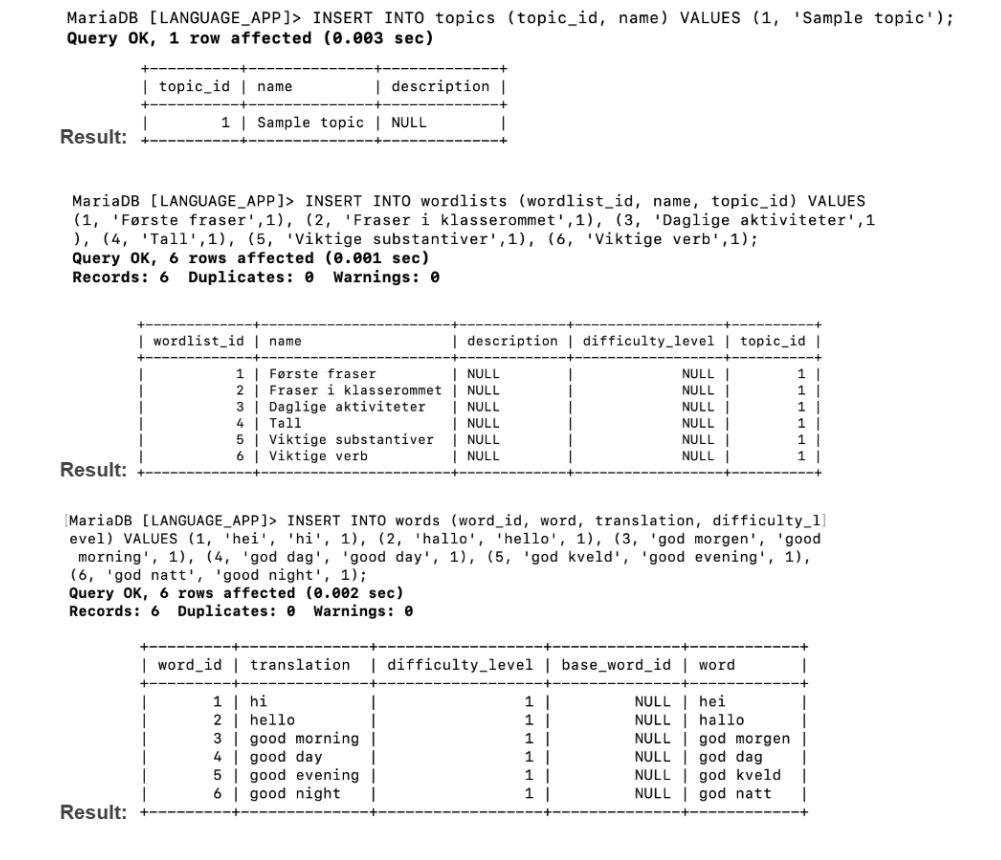
\includegraphics[width=0.8\linewidth]{3ans.png}
    \label{fig:placeholder}
\end{figure}


\begin{figure}[H]
    \centering
    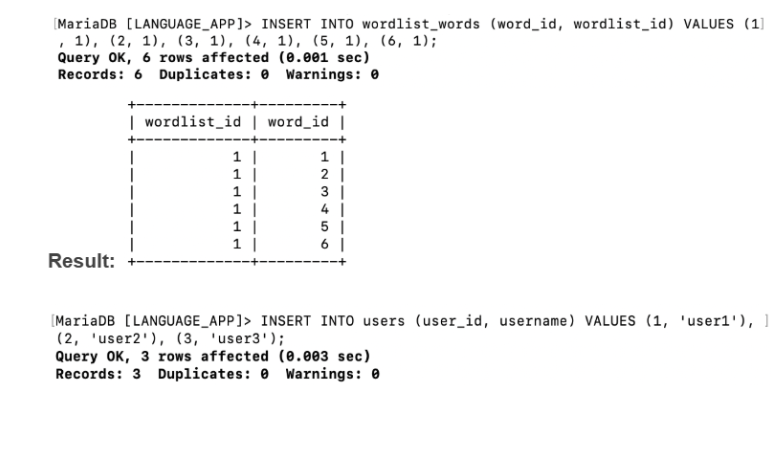
\includegraphics[width=0.8\linewidth]{4ans.png}
    \label{fig:placeholder}
\end{figure}

\begin{figure}[H]
    \centering
    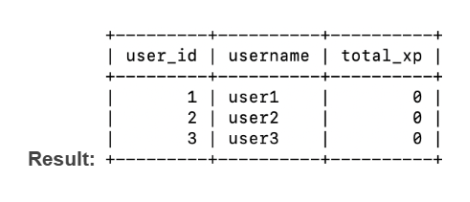
\includegraphics[width=0.4\linewidth]{ans5.png}
    \label{fig:placeholder}
\end{figure}

\paragraph*{{Report SQL QUERY}}
\noindent
\begin{figure}[H]
    \centering
    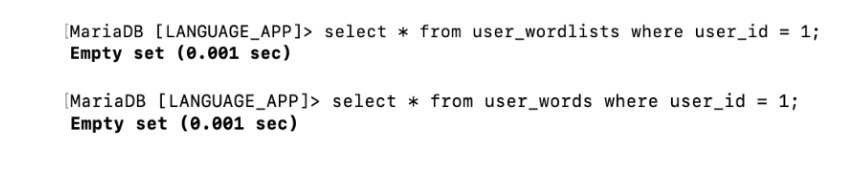
\includegraphics[width=0.8\linewidth]{ans8.png}
    \label{fig:placeholder}
\end{figure}

\clearpage
\paragraph*{{SQL INSERT statements for the use case}}
\noindent
\begin{figure}[H]
    \centering
    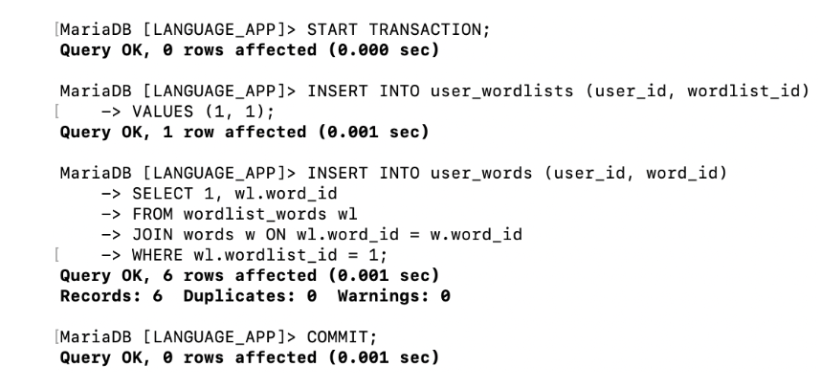
\includegraphics[width=0.8\linewidth]{ans7.png}
    \label{fig:placeholder}
\end{figure}


\paragraph*{{Report after the execution of SQL INSERT}}
\noindent
\begin{figure}[H]
    \centering
    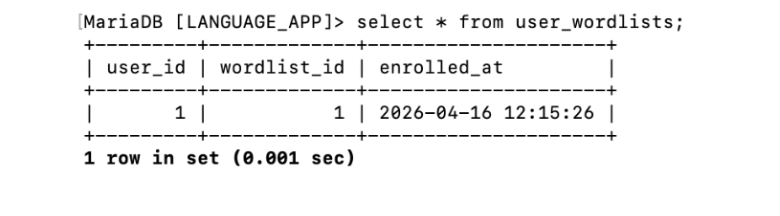
\includegraphics[width=0.8\linewidth]{ans9.png}
    \label{fig:placeholder}
\end{figure}

\begin{figure}[H]
    \centering
    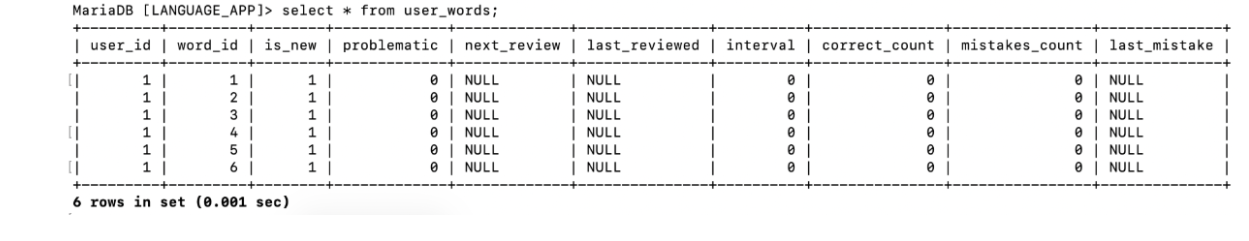
\includegraphics[width=0.8\linewidth]{ans100.png}
\end{figure}






\newpage

\subsection{Individual - Student 3}
\studentthree
%%%%%%%%%%%%%%%%%%%%%%%%%%%%%%%%%%%%%%%%%
\subsubsection{Use Case Definition and Design}
\textcolor{gray}{

The use case is reviewing the words by user, Version 3 (user\_words table: each user can have many words assigned and each word can be assigned to many users)


\paragraph*{Textual Description}
\textbf{Use Case Name (weak entity/IS-A relationship/many-to-many): Word review process}
\\
\textbf{Trigger:}    User answers a question/translates the word and clocks on next during Review Session                                       
\\
\textbf{Preconditions:}    
\begin{itemize}
    \item User is exists in the database
\item User has at least one word assigned
\item User has at least 1 word in \item user\_words pending review
\item User is logged in

\end{itemize}

\\
\textbf{Main Flow:} 
\begin{enumerate}
    \item 	User clicks on Review button
\item The first word is displayed
\item The user reviews the word, result is marked as correct/incorrect
\item 	Frontend sends to the Backend the word\_id, the correct/incorrect flag, and the session\_id
\item The interval and the next\_review\_date is calculated from the data received from the frontend and retrieved from DB.
\item On DB level:
\begin{itemize}
\item problematic, last\_mistake, fields for the word are updated
\item correct\_count, mistake\_count in Word table are incremented
\item	interval and review\_date are updated
\item	last\_reviewed is set to NOW()
\item	if is\_new  == 1, set to 0
\item	The words\_count field in the learning\_session table is incremented

\end{itemize}

\item 	Success message displays
\item 	If it was the last word, end the session, else - repeat p.3-7

\end{enumerate}

\\
\textbf{Postconditions:}
\begin{itemize}
    \item The timestamps of the user\_word table are actualized, so user can continue learning/reviewing the next time.
    \item Progress of user is documented
\end{itemize}

\\
\textbf{Entities:}
User, Learning Session, Word
\\

\paragraph*{Graphical Representation}



\begin{center}
\begin{figure}[H]
    \centering
    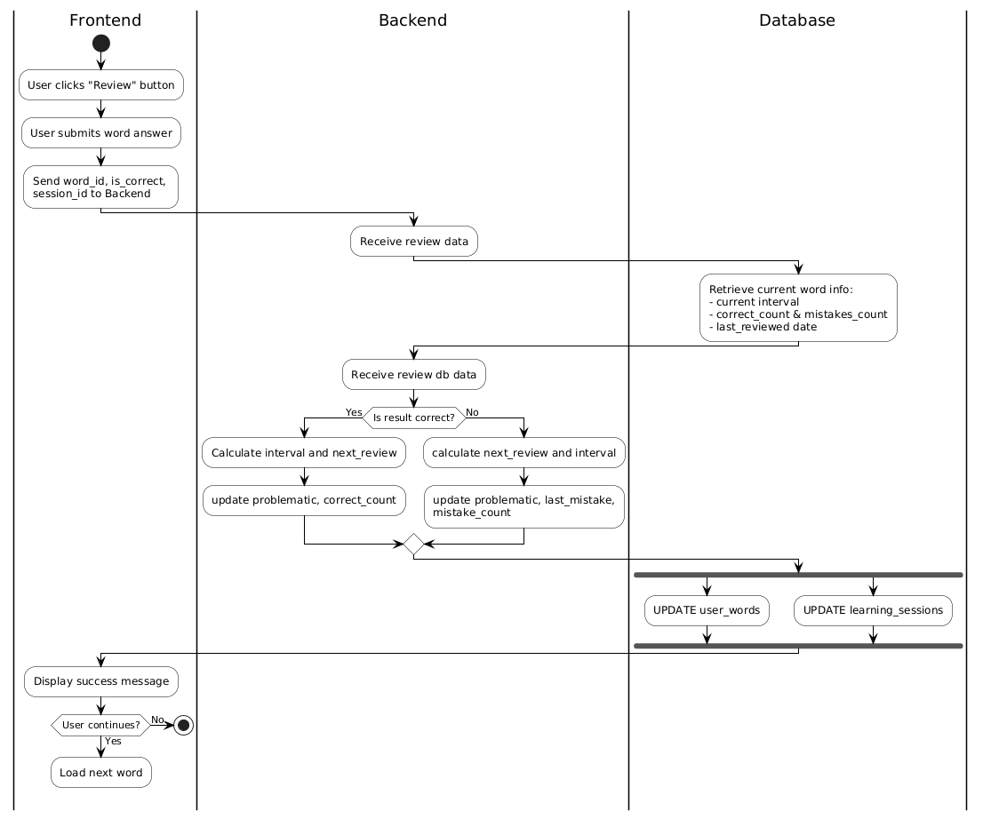
\includegraphics[width=0.8\textwidth]{anna_activtx.png}
    \caption{Activity Diagram from Use Case 3}
    \label{fig:activity-diagram}
\end{figure}
\end{center}

%%%%%%%%%%%%%%%%%%%%%%%%%%%%%%%%%%%%%%%%%
%%%%%%%%%%%%%%%%%%%%%%%%%%%%%%%%%%%%%%%%%
\subsubsection{Analytics Report}
\paragraph*{Concept}

This analytical report provides statistic on words which were learned by user over the last review session, as well as some deeper statistics of a learning progress of specific words learned during the last review session, showing how many times the word was recognised/translated correct, and how much mistakes for this word were made over the whole learning history. This report is updated after each review session is finished to see some useful insights on it.

Entities Involved :
\begin{enumerate}
    \item Users
    \item Words
    \item Topics
    \item Learning\_Sessions
\end{enumerate}







\begin{figure}
    \centering
    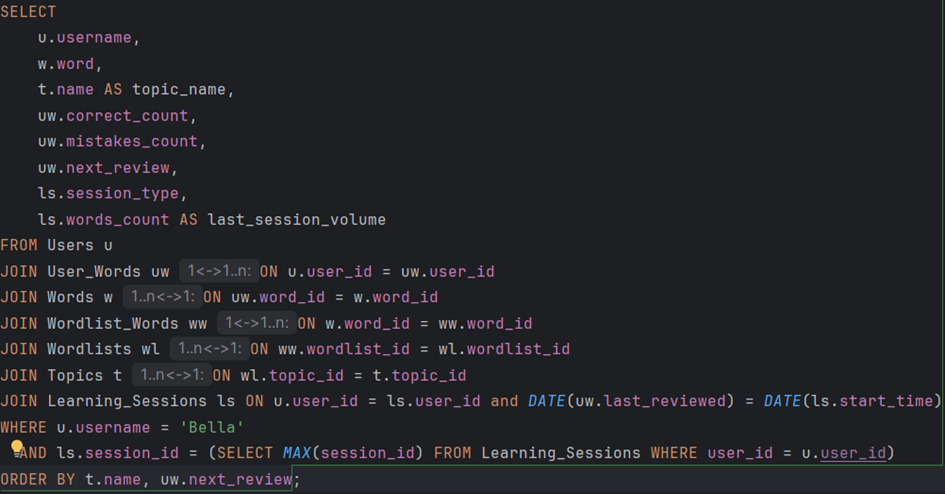
\includegraphics[width=0.7\linewidth]{image.png}
    \label{fig:placeholder}
\end{figure}


\paragraph*{Proof of Concept }
\textcolor{gray}{
Add screenshots and descriptions of executing your analytics report.
}

\begin{figure}
    \centering
    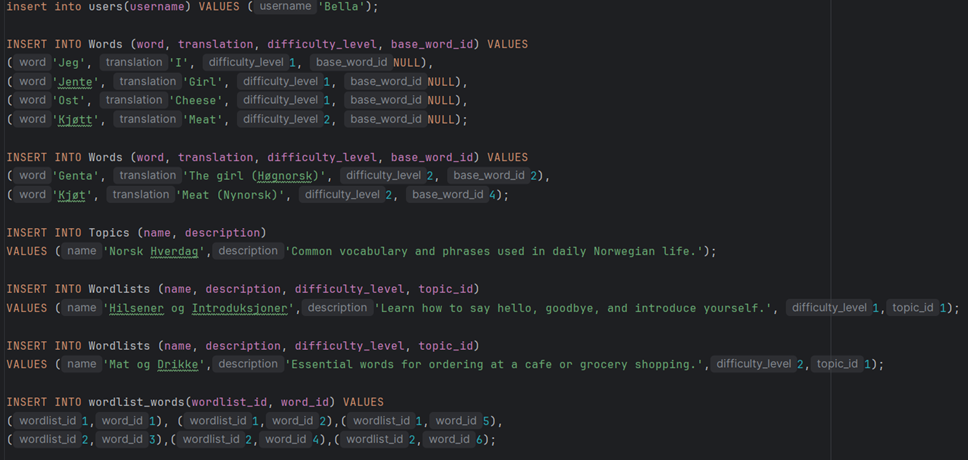
\includegraphics[width=0.7\linewidth]{1an.png}
    \label{fig:placeholder}
\end{figure}

\begin{figure}
    \centering
    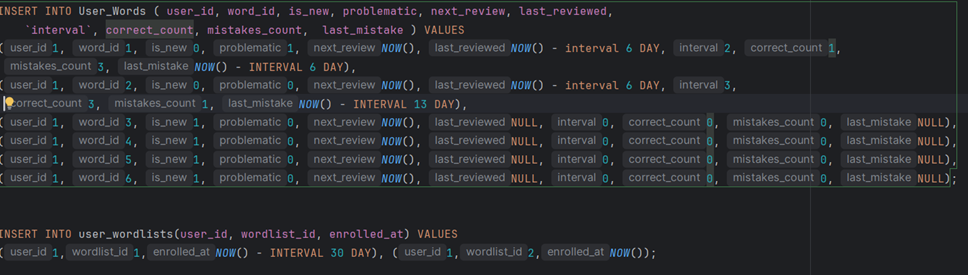
\includegraphics[width=0.7\linewidth]{2ann.png}
    \caption{inserting the dummy data}
    \label{fig:placeholder}
\end{figure}

\begin{figure}
    \centering
    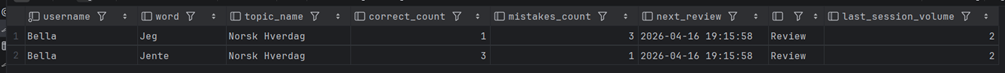
\includegraphics[width=0.7\linewidth]{3ann.png}
    \caption{Before the Use Case execution}
    \label{fig:placeholder}
\end{figure}


\begin{figure}
    \centering
    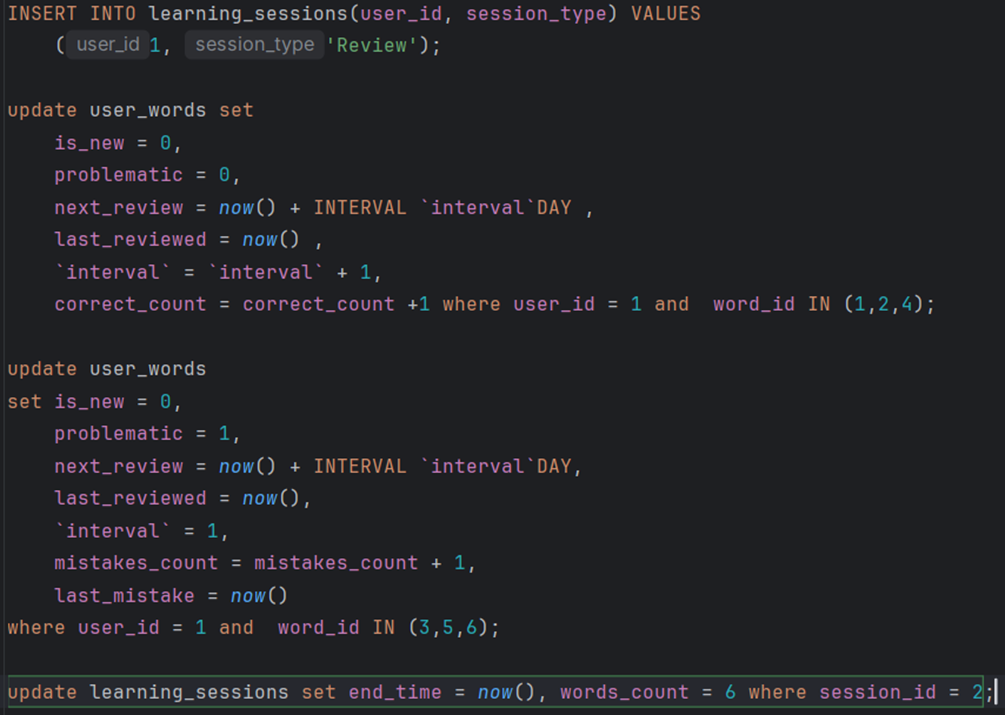
\includegraphics[width=0.7\linewidth]{4ann.png}
    \caption{Use Case execution}
    \label{fig:placeholder}
\end{figure}

\begin{figure}
    \centering
    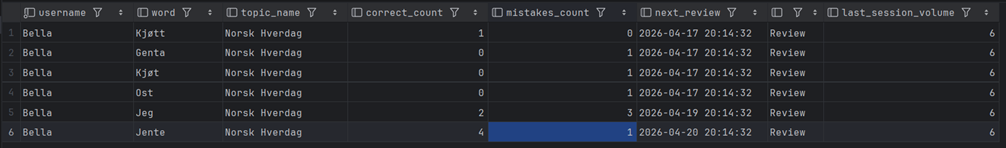
\includegraphics[width=0.7\linewidth]{5ann.png}
    \caption{After the Use Case execution}
    \label{fig:placeholder}
\end{figure}

\newpage

\subsection{Summary}
\begin{table}[H]
\resizebox{\textwidth}{!}{
\begin{tabular}{|l|l|l|l|l|}
\hline
\rowcolor[HTML]{93C47D} 
\makecell{\textbf{Type} \\ \color[HTML]{808080} \tiny Read or write}  & 
\makecell{\textbf{Operation} \\ \color[HTML]{808080} \tiny Name of a functions}  & 
\makecell{\textbf{Information} \\ \color[HTML]{808080} \tiny Involved entities}  & 
\makecell{\textbf{Frequency } \\ \color[HTML]{808080} \tiny The rate of calling the operation}  & 
\makecell{\textbf{Criticality} \\ \color[HTML]{808080} \tiny High/Medium/Low}  \\ \hline

Write & Assign Word to Wordlist & User, Wordlist, Word, Wordlist\_Word & Medium & Medium \\ \hline

Write & Assign Wordlist to User & User, Wordlist, User\_Wordlist, User\_Word & Low & High \\ \hline

Write & Review Word / Update Progress & User, Word, User\_Word, Learning\_Session & High & High \\ \hline


\end{tabular}
}
\end{table}


\end{document}